% !TEX root = ../thesis.tex

\chapter{System and Methodology}
\label{chp:method}

\section{Robot Platform: B2Z1}
\label{sec:platform}

The hardware platform used in this project is the Unitree B2+Z1
loco-manipulator, illustrated schematically in
Figure~\ref{fig:robot_dof}.
The \textbf{Unitree B2} is a quadrupedal robot with four three-DOF legs
(hip abduction/adduction, hip flexion/extension, knee flexion/extension),
giving 12 leg DOFs in total.
The B2 is designed for industrial and field deployment, with a rated payload
of approximately 5\,kg in manipulation and a body mass around 60\,kg,
substantially heavier than the Go1 (12\,kg).
The \textbf{Unitree Z1} is a six-DOF serial manipulator---
\texttt{z1\_waist} (base rotation),
\texttt{z1\_shoulder} (shoulder lift),
\texttt{z1\_elbow} (elbow flexion),
\texttt{z1\_wrist\_angle} (wrist pitch),
\texttt{z1\_forearm\_roll} (forearm roll),
\texttt{z1\_wrist\_rotate} (wrist rotation)---plus one underactuated
gripper DOF (\texttt{z1\_jointGripper}).
The arm is mounted at the front of the B2 body, with its base at
approximately $h_\text{mount} = 0.38$\,m above the ground when the
quadruped stands at its nominal height.

Together, the robot has \textbf{19 physical DOFs}; however, the RL action
space covers only 18 DOFs (12 leg + 6 arm).
The gripper DOF~18 has zero PD gains in training and must be controlled
separately by direct DOF state injection.
Table~\ref{tab:dof_structure} summarises the DOF indexing.

\begin{table}[htbp]
  \centering
  \caption{DOF indexing of the B2Z1 system (19 DOFs total).}
  \label{tab:dof_structure}
  \renewcommand{\arraystretch}{1.1}
  \begin{tabular}{clll}
    \toprule
    \textbf{DOF index} & \textbf{Joint name} & \textbf{Type} &
    \textbf{Kp / Kd} \\
    \midrule
    0--2   & FL hip, thigh, calf  & Leg & 200 / 20 \\
    3--5   & FR hip, thigh, calf  & Leg & 200 / 20 \\
    6--8   & RL hip, thigh, calf  & Leg & 200 / 20 \\
    9--11  & RR hip, thigh, calf  & Leg & 200 / 20 \\
    12     & z1\_waist            & Arm & 40 / 2   \\
    13     & z1\_shoulder         & Arm & 60 / 6   \\
    14     & z1\_elbow            & Arm & 60 / 6   \\
    15     & z1\_wrist\_angle     & Arm & 20 / 1   \\
    16     & z1\_forearm\_roll    & Arm & 20 / 1   \\
    17     & z1\_wrist\_rotate    & Arm & 20 / 1   \\
    18     & z1\_jointGripper     & Gripper & 0 / 0 (state injection) \\
    \bottomrule
  \end{tabular}
\end{table}

\begin{figure}[htbp]
  \centering
  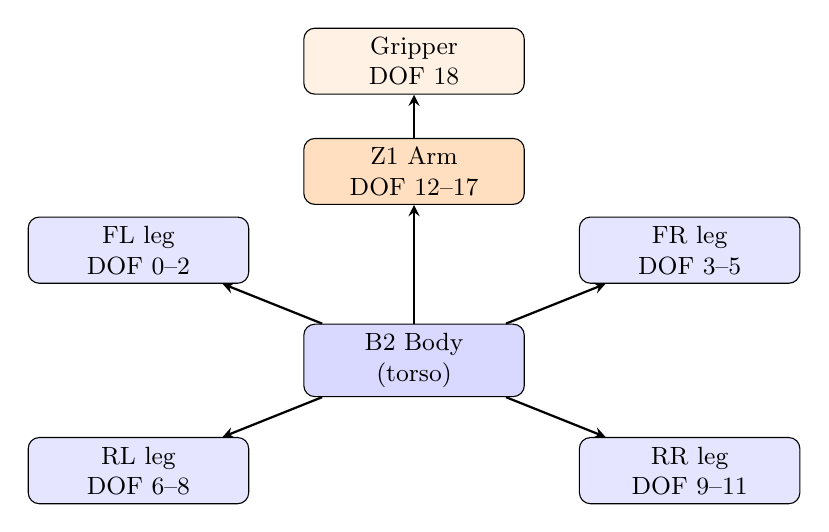
\begin{tikzpicture}[
      box/.style={draw,rounded corners,minimum width=2.8cm,
                  minimum height=0.8cm,align=center,font=\small},
      arr/.style={->,>=stealth,thick}
    ]
    % Quadruped body
    \node[box, fill=blue!15] (body) at (0,0) {B2 Body\\(torso)};
    % Four legs
    \node[box, fill=blue!10] (fl) at (-3.5, 1.4) {FL leg\\DOF 0--2};
    \node[box, fill=blue!10] (fr) at ( 3.5, 1.4) {FR leg\\DOF 3--5};
    \node[box, fill=blue!10] (rl) at (-3.5,-1.4) {RL leg\\DOF 6--8};
    \node[box, fill=blue!10] (rr) at ( 3.5,-1.4) {RR leg\\DOF 9--11};
    % Arm
    \node[box, fill=orange!25] (arm) at (0, 2.4) {Z1 Arm\\DOF 12--17};
    \node[box, fill=orange!10] (grip) at (0, 3.8) {Gripper\\DOF 18};
    % Arrows
    \draw[arr] (body) -- (fl);
    \draw[arr] (body) -- (fr);
    \draw[arr] (body) -- (rl);
    \draw[arr] (body) -- (rr);
    \draw[arr] (body) -- (arm);
    \draw[arr] (arm)  -- (grip);
  \end{tikzpicture}
  \caption{DOF structure of the B2Z1 system.  Blue boxes: quadruped legs
           (torque-controlled). Orange boxes: Z1 arm (position-controlled)
           and gripper (state injection, no PD).}
  \label{fig:robot_dof}
\end{figure}

\section{Simulation Environment}
\label{sec:sim}

All training and demonstrations use NVIDIA IsaacGym~\cite{makoviychuk2021isaac},
a GPU-accelerated rigid-body physics simulator.
The key simulation parameters are:
physics time-step $\Delta t = 0.005$\,s,
control decimation $d = 4$ (policy runs at 50\,Hz),
$N_\text{envs} = 4096$ parallel environments during training and
$N_\text{envs} = 1$ during demonstration.
The PhysX solver uses 4 position and 1 velocity iterations per step.

The robot URDF is loaded from
\texttt{resources/robots/b2z1/urdf/b2z1.urdf}.
During training, domain randomisation is applied to friction
($\mu \in [0.5, 1.25]$), base added mass ($[-2, 2]$\,kg), action delay
(6 timestep lag), and random external pushes (every 15\,s, up to 1\,m/s).
These perturbations improve policy robustness and facilitate sim-to-real
transfer.

\section{Decentralised Two-Policy Architecture}
\label{sec:architecture}

RoboDuet employs two independent policies that are trained concurrently but
without explicit inter-policy communication.

\subsection{Dog Policy \texorpdfstring{$\pi_\text{dog}$}{pi-dog}}

The dog policy $\pi_\text{dog}$ outputs 12-dimensional leg joint position
targets.
Its observation history has 56 proprioceptive features per timestep
retained over 30 steps (1680-dimensional history input total) plus a
2-dimensional privileged observation.
The dog policy is based on the WTW gait-conditioned
architecture~\cite{margolis2023walk} and is trained with locomotion rewards
(velocity tracking, orientation, contact shaping) as well as whole-body
coupling rewards (orientation heuristic, hip action penalty).
In all our demonstrations, locomotion velocity commands are set to zero so
that the dog policy acts as a \emph{standing stabiliser}.

\subsection{Arm Policy \texorpdfstring{$\pi_\text{arm}$}{pi-arm}}

The arm policy $\pi_\text{arm}$ outputs an 8-dimensional vector:
6 arm joint position offsets plus 2 planned end-effector velocity targets.
Its architecture is described in detail in Section~\ref{sec:arm_policy}.

\section{Arm Command Space}
\label{sec:commands}

The arm policy receives three primary scalar commands sampled from the
ranges in Table~\ref{tab:arm_commands}:

\begin{table}[htbp]
  \centering
  \caption{Arm command parameters and ranges.}
  \label{tab:arm_commands}
  \renewcommand{\arraystretch}{1.1}
  \begin{tabular}{cllll}
    \toprule
    \textbf{Symbol} & \textbf{Name} & \textbf{Range} &
    \textbf{Unit} & \textbf{Interpretation} \\
    \midrule
    $l$    & Reach length & $[0.30,\; 0.77]$ & m    &
             Desired EE distance from arm base \\
    $p$    & Pitch angle  & $[-0.45\pi,\; 0.45\pi]$ & rad &
             Elevation of EE above arm base plane \\
    $\psi$ & Yaw angle    & $[-\pi/2,\; \pi/2]$ & rad &
             Lateral azimuth of EE in body frame \\
    $\alpha,\beta,\gamma$ & EE roll/pitch/yaw & $\pm$60--75$^\circ$ & rad &
             Optional 6D pose orientation targets \\
    \bottomrule
  \end{tabular}
\end{table}

The desired end-effector world position corresponding to commands
$(l, p, \psi)$ is:
\begin{equation}
  \mathbf{p}_\text{EE} =
  \begin{pmatrix}
    l\cos p\cos\psi \\
    l\cos p\sin\psi \\
    l\sin p + h_\text{mount}
  \end{pmatrix}
  \label{eq:ee_pos}
\end{equation}
where $h_\text{mount} = 0.38$\,m is the height of the arm base above the
ground.
For our demonstrations we use $l = 0.55$\,m, $p = 0.25$\,rad,
$\psi = 0$, giving a predicted reach position of
$(0.533, 0, 0.516)$\,m in the world frame
(\emph{i.e.}\ 0.533\,m forward, 0.516\,m above the ground).

\section{Observation and Action Spaces}
\label{sec:obs}

\subsection{Arm Policy Observation Space}
\label{sec:arm_obs}

The arm policy observes 20 proprioceptive features at each timestep.
Based on the framework configuration (\texttt{arm\_num\_observations~=~26-6~=~20}),
these 20 features consist of the quantities listed in
Table~\ref{tab:arm_obs}.

\begin{table}[htbp]
  \centering
  \caption{Arm policy observation vector (20 dimensions per step;
           30-step history = 600-dim input).}
  \label{tab:arm_obs}
  \renewcommand{\arraystretch}{1.1}
  \begin{tabular}{lcc}
    \toprule
    \textbf{Observation} & \textbf{Dims} & \textbf{Scale} \\
    \midrule
    Arm joint positions (DOF 12--17 offset from default) & 6  & 1.0 \\
    Arm joint velocities (DOF 12--17)                    & 6  & 0.05 \\
    Arm commands $(l, p, \psi, \alpha, \beta, \gamma)$   & 6  & 1.0 \\
    Body roll angle                                       & 1  & 1.0 \\
    Body pitch angle                                      & 1  & 1.0 \\
    \midrule
    \textbf{Total}                                        & \textbf{20} & -- \\
    \bottomrule
  \end{tabular}
\end{table}

The full input to the adaptation module and history encoder is
a 600-dimensional vector formed by concatenating 30 consecutive
observation steps.
Additionally, a 9-dimensional privileged observation is available
during training (friction, base mass, CoM displacement, motor parameters,
\emph{etc.}).

\subsection{Action Space}
\label{sec:actions}

The arm policy outputs 8 values: 6 joint position offsets $\Delta q_\text{arm}
\in [-1, 1]$ (applied with scale 0.5) for DOFs 12--17, and 2 planned
velocity targets for the end-effector (bounded by $\tanh$ to $[-1, 1]$).
The dog policy outputs 12 joint position offsets $\Delta q_\text{leg}$ for
DOFs 0--11 with the same 0.5 scaling.
The full 18-dimensional combined action $a = [\Delta q_\text{leg};
\Delta q_\text{arm}]$ is then passed through the mixed-mode (M) controller.

\section{Mixed-Mode Controller}
\label{sec:control}

The mixed-mode (``M'') controller applies different actuation primitives to
the two subsystems:
\begin{equation}
  \boldsymbol{\tau}_\text{leg} =
  K_p^\text{leg}\bigl(q_\text{target} - q\bigr)
  - K_d^\text{leg}\,\dot{q},
  \quad
  K_p^\text{leg} = 200,\quad K_d^\text{leg} = 20
  \label{eq:leg_torque}
\end{equation}
\begin{equation}
  \theta_\text{arm,target} = q_\text{default} + \Delta q_\text{arm}
  \quad\text{(position target sent to actuator PD)}
  \label{eq:arm_pos}
\end{equation}
with arm joint-specific gains:
$K_p^\text{arm} = [40, 60, 60, 20, 20, 20]$,
$K_d^\text{arm} = [2, 6, 6, 1, 1, 1]$.
The gripper (DOF~18) has $K_p = K_d = 0$; it is controlled by directly
writing its position into the IsaacGym DOF state tensor at each step,
bypassing the PD layer entirely.

\section{Reward Functions}
\label{sec:rewards}

The reward is split into dog rewards (fed to $\pi_\text{dog}$) and arm
rewards (fed to $\pi_\text{arm}$); walking rewards are excluded from
$r_\text{arm}$.
Table~\ref{tab:rewards} lists all active reward terms with their scales.

\begin{table}[htbp]
  \centering
  \caption{Reward terms used in B2Z1 training.  Terms marked $\dagger$
           contribute to the arm reward only; all others contribute to both.}
  \label{tab:rewards}
  \renewcommand{\arraystretch}{1.1}
  \begin{tabular}{lll}
    \toprule
    \textbf{Term} & \textbf{Scale} & \textbf{Formula / Notes} \\
    \midrule
    \multicolumn{3}{l}{\textit{Locomotion (dog only)}} \\
    $r_\text{lin\_vel}$         & $+1.0$ &
      $\exp\!\left(-\tfrac{(v_x - v_x^*)^2}{\sigma}\right)$ \\
    $r_\text{ang\_vel}$         & $+0.5$ &
      $\exp\!\left(-\tfrac{(\omega_z - \omega_z^*)^2}{\sigma}\right)$ \\
    \midrule
    \multicolumn{3}{l}{\textit{Whole-body (dog + arm)}} \\
    $r_\text{manip\_tracking}^\dagger$
                                & $+1.0$ &
      $\exp\!\bigl(-(3\,\varepsilon_\text{lpy} +
                      1\,\varepsilon_\text{rpy})\bigr)$;
      $\varepsilon_\text{lpy}=\|(\hat{l},\hat{p},\hat{\psi}) -
                                (l^*,p^*,\psi^*)\|/\Delta_\text{lpy}$ \\
    $r_\text{orient\_heuristic}$& $-2.0$ & Body tilt penalty \\
    $r_\text{orient\_control}$  & $-10.0$& Body orientation error \\
    $r_\text{hip\_l2}$          & $-0.05$& $\|\Delta q_\text{hip}\|^2$,
      penalises lateral hip excursions \\
    $r_\text{control\_limits}^\dagger$
                                & $-5.0$ & Joint limit violation penalty \\
    $r_\text{smooth1}^\dagger$  & $-0.1$ &
      $\|q_\text{target}^t - q_\text{target}^{t-1}\|^2$ \\
    $r_\text{loco\_energy}$     & $-4\times10^{-5}$ &
      $\|\boldsymbol{\tau}_\text{leg}\|^2$ \\
    $r_\text{arm\_energy}^\dagger$
                                & $-4\times10^{-5}$ &
      $\|\boldsymbol{\tau}_\text{arm}\|^2$ \\
    \bottomrule
  \end{tabular}
\end{table}

The manipulation tracking reward $r_\text{manip\_tracking}$ is the primary
learning signal for the arm policy.
It penalises deviation of the measured end-effector spherical coordinates
$(\hat{l},\hat{p},\hat{\psi})$ from the commanded targets
$(l^*,p^*,\psi^*)$, weighted by the command range $\Delta_\text{lpy}$.
The weighting of 3:1 between position error ($\varepsilon_\text{lpy}$) and
orientation error ($\varepsilon_\text{rpy}$) reflects the relative
importance of placing the end-effector at the correct location
over achieving a specific wrist orientation.

\section{Arm Policy Architecture}
\label{sec:arm_policy}

The arm policy implements the \emph{teacher-student} adaptation architecture
introduced by Kumar~\emph{et al.}~\cite{kumar2021rma} and used in RoboDuet.
It consists of three learned modules, depicted in Figure~\ref{fig:arm_arch}:

\begin{enumerate}
  \item \textbf{Adaptation Module} $\phi$:
        encodes the full 600-dimensional observation history into a
        9-dimensional latent vector $z \in \mathbb{R}^9$ approximating
        the privileged environment information.
        Architecture: $[600 \to 256 \to 128 \to 9]$ with ELU activations.
  \item \textbf{History Encoder} $\xi$:
        encodes the 580-dimensional \emph{past} window
        (history minus the current observation, \emph{i.e.}\ 600~$-$~20) into
        a 128-dimensional history latent $h \in \mathbb{R}^{128}$.
        Architecture: $[580 \to 512 \to 256 \to 128]$ with ELU activations.
  \item \textbf{Actor} $\pi$:
        maps the concatenated vector $(o_t, z, h) \in \mathbb{R}^{157}$
        to 8 action logits.
        Architecture: $[157 \to 512 \to 256 \to 128 \to 8]$ with ELU.
\end{enumerate}

A parallel \textbf{Critic} network mirrors the actor structure but outputs
a scalar value estimate $V \in \mathbb{R}$ for PPO training.
The last two outputs of the actor ($\Delta 7$, $\Delta 8$) are passed through
$\tanh$ to bound them in $[-1, 1]$ before being used as planned velocity
targets.

\begin{figure}[htbp]
  \centering
  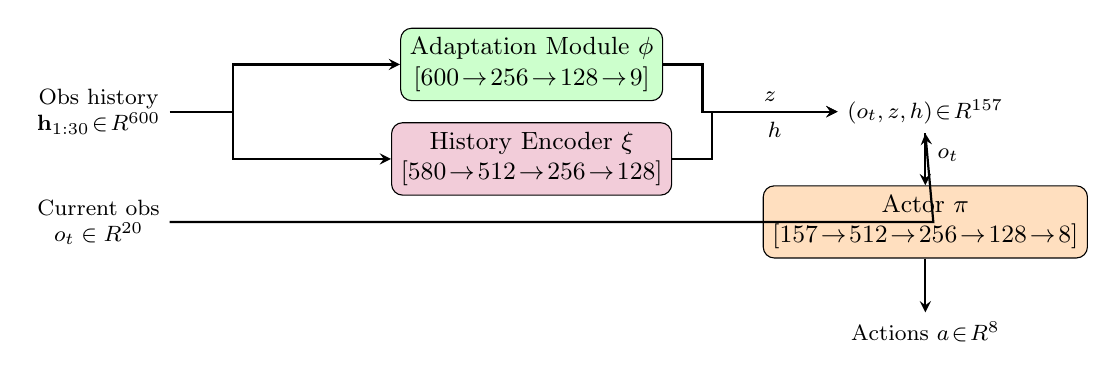
\begin{tikzpicture}[
      module/.style={draw,rounded corners,minimum width=3.2cm,
                     minimum height=0.9cm,align=center,font=\small},
      data/.style={font=\footnotesize,align=center},
      arr/.style={->,>=stealth,thick}
    ]
    % Input
    \node[data] (hist) at (0,  0) {Obs history\\$\mathbf{h}_{1:30}\!\in\!\mathbb{R}^{600}$};
    \node[data] (obs)  at (0, -1.4) {Current obs\\$o_t \in\mathbb{R}^{20}$};
    % Modules
    \node[module, fill=green!20]   (adapt)  at ( 5.5,  0.6)
         {Adaptation Module $\phi$\\$[600\!\to\!256\!\to\!128\!\to\!9]$};
    \node[module, fill=purple!20]  (histenc) at ( 5.5, -0.6)
         {History Encoder $\xi$\\$[580\!\to\!512\!\to\!256\!\to\!128]$};
    % Concat
    \node[data] (cat) at (10.5,0) {$(o_t, z, h)\!\in\!\mathbb{R}^{157}$};
    % Actor
    \node[module, fill=orange!25]  (actor)  at (10.5,-1.4)
         {Actor $\pi$\\$[157\!\to\!512\!\to\!256\!\to\!128\!\to\!8]$};
    \node[data] (act) at (10.5,-2.8) {Actions $a\!\in\!\mathbb{R}^8$};
    % Arrows
    \draw[arr] (hist.east) -- ++(0.8,0) |- (adapt.west)
               node[midway,above,font=\footnotesize]{};
    \draw[arr] (hist.east) -- ++(0.8,0) |- (histenc.west);
    \draw[arr] (adapt.east)   -- ++(0.5,0) |- (cat.west)
               node[near end,above,font=\footnotesize]{$z$};
    \draw[arr] (histenc.east) -- ++(0.5,0) |- (cat.west)
               node[near end,below,font=\footnotesize]{$h$};
    \draw[arr] (obs.east)     -- ++(9.7,0) -- (cat.south)
               node[near end,right,font=\footnotesize]{$o_t$};
    \draw[arr] (cat) -- (actor);
    \draw[arr] (actor) -- (act);
  \end{tikzpicture}
  \caption{Arm policy architecture.  The adaptation module $\phi$ infers a
           9-dim environment latent $z$ from the full observation history;
           the history encoder $\xi$ extracts a 128-dim temporal feature $h$
           from the past window.  The actor concatenates $(o_t, z, h)$ and
           outputs 8 actions.}
  \label{fig:arm_arch}
\end{figure}

\section{Training via Proximal Policy Optimisation}
\label{sec:ppo}

Both policies are trained with PPO~\cite{schulman2017ppo} in the on-policy
regime with $N_\text{envs}=4096$ parallel environments.
The two-stage training curriculum is:
\begin{enumerate}
  \item \textbf{Pre-training stage} (switch closed): each policy is
        pre-trained in isolation using zero actions from the other agent,
        so the dog policy learns to stand and walk while the arm policy
        learns basic reaching.
  \item \textbf{Hybrid stage} (switch open): both policies run
        simultaneously.  The shared body dynamics couple them, and each
        policy receives its own reward signal, converging to a cooperative
        equilibrium.
\end{enumerate}
The global switch flag \texttt{global\_switch.switch\_open} controls which
stage is active; for all our demonstrations it is set to \texttt{True},
meaning the arm policy uses live arm-command observations rather than
zero-padded inputs.
Training was performed on a server equipped with an NVIDIA RTX 4090 (24\,GB)
GPU for approximately 200 million environment steps over $\sim$24 hours.

\section{Adaptation from Go1+Z1 to B2+Z1}
\label{sec:adaptation}

The original RoboDuet codebase targets the lighter Unitree Go1 quadruped.
Adapting it to B2+Z1 required the following changes:

\begin{enumerate}
  \item \textbf{URDF}: replaced \texttt{go1z1.urdf} with
        \texttt{b2z1.urdf} in \texttt{config\_asset.py}.  The B2 has wider
        stance, heavier links, and different joint offsets than the Go1.
  \item \textbf{Default joint angles}: updated default standing pose in
        \texttt{config\_go1.py} (hip, thigh, calf angles) to match the B2
        natural stand.
  \item \textbf{PD gains}: leg gains were increased from
        $(K_p, K_d) = (35, 1)$ (Go1 factory values) to $(200, 20)$ to
        provide sufficient torque bandwidth for the heavier B2 body.
  \item \textbf{Arm gains}: unchanged from Go1+Z1 since the Z1 arm is
        identical; $K_p = [40, 60, 60, 20, 20, 20]$,
        $K_d = [2, 6, 6, 1, 1, 1]$.
  \item \textbf{Observation dimensions}: \texttt{num\_observations = 63},
        \texttt{num\_privileged\_obs = 9} confirmed to match the loaded
        checkpoint architecture by verifying forward-pass dimensions.
  \item \textbf{Nominal body height}: the B2 stands at
        $h \approx 0.45$\,m (vs.~Go1's $\approx 0.32$\,m), so the arm mount
        height $h_\text{mount}$ was updated in the demonstration scripts.
\end{enumerate}

The authors of RoboDuet claimed zero-shot transfer across quadrupeds of
``similar morphology and physical dimensions''; while B2 is significantly
heavier than Go1, the arm geometry and Z1 kinematic structure are identical,
and the adaptation steps above are sufficient for the arm policy to transfer
successfully.

\section{Grasp-and-Lift Demonstration Pipeline}
\label{sec:demo}

The final demonstration (\texttt{gen\_grasp\_fixedbase\_success.py}) required solving
a non-trivial engineering challenge: how to make the simulation \emph{appear}
to grasp and lift an object without physical contact simulation.

\subsection{Why Scripted Arm Angles Fail}

Early approaches (v1--v6) attempted to drive the arm to a scripted joint
configuration $[\Delta q_\text{waist},\ldots] = [0,-4,4,0,0,0]$
(approximately forward-reach pose).
Post-hoc forward kinematics analysis showed this pose places the gripper at
$x \approx -0.085$\,m (\emph{behind} the robot), not forward.
This is because the B2Z1 arm base orientation differs from the Go1Z1, and
na\"ively copying joint angles produces an unintended reach direction.

\subsection{Policy-Based Forward Reach and Gripper Calibration}

Instead, setting the arm commands to
$(l, p, \psi) = (0.55, 0.25, 0.0)$ and running the arm policy produces a
stable reach in the forward direction.
Before recording, the script runs an additional 60 warm-up steps at
$p = p_\text{low} = 0.25$ with the base link fixed, then reads the
\emph{actual} gripperMover rigid-body position from the IsaacGym state
tensor (\texttt{rbs[GRIP\_BODY\_IDX]}).
This calibrated position is used as
$\mathbf{p}_\text{reach} \in \mathbb{R}^3$ (the box placement target), so
that the box is placed exactly where the gripper arrives---not at an
analytical approximation.

\subsection{Hybrid Box Teleportation Strategy}

Simulating a visible grasp and lift without rigid-body contact was
achieved by teleporting a kinematic box at each step:
\begin{enumerate}
  \item Spawn a $6\,\text{cm}\times6\,\text{cm}\times6\,\text{cm}$
        \textbf{green} kinematic box
        (\texttt{fix\_base\_link = True, disable\_gravity = True}) at a
        hidden position $(0, 0, -10)$\,m during the warm-up phase.
  \item Place the box at the calibrated reach position
        $\mathbf{p}_\text{reach}$ from the first recorded frame onward.
  \item After the gripper closes (DOF~18 ramped $0 \to -0.80$\,rad),
        enter the LIFT phase.  Rather than following the analytical EE
        trajectory (which was found to move the arm primarily sideways,
        yielding negligible height gain), a \emph{hybrid} strategy is used:
        \begin{equation}
          \mathbf{p}_\text{box}(t) =
          \begin{pmatrix}
            x_\text{grip}(t) \\
            y_\text{grip}(t) \\
            \text{lerp}\!\bigl(
              p_\text{reach,z},\;
              p_\text{reach,z} + \Delta z,\;
              \tfrac{t - T_\text{lift}}{N_\text{lift}}
            \bigr)
          \end{pmatrix}
          \label{eq:hybrid_lift}
        \end{equation}
        where $(x_\text{grip}(t), y_\text{grip}(t))$ is the live gripperMover
        XY position read from the state tensor at each step, and
        $\Delta z = 0.30$\,m is the target lift height.
        The XY component keeps the box aligned with the gripper as the arm
        sweeps sideways during pitch transition; the independently animated
        Z component ensures a clearly visible 30\,cm upward trajectory.
  \item During the HOLD2 phase the box XY continues to track the gripper
        while Z is held fixed at $p_\text{reach,z} + \Delta z$.
\end{enumerate}

The maximum box displacement per step in the Z direction is:
\[
  d_\text{max} = \frac{\Delta z}{N_\text{lift}} \times 1000
  = \frac{300\,\text{mm}}{170} \approx 1.76\;\text{mm/step}
\]
which is well below the IsaacGym interpenetration threshold
($\approx$5\,mm), and the kinematic box reacts to no contact forces,
making it safe to teleport at each step.

The full phase sequence is listed in Table~\ref{tab:phases}.

\begin{table}[htbp]
  \centering
  \caption{Phase sequence of the grasp-and-lift demonstration (v7).}
  \label{tab:phases}
  \renewcommand{\arraystretch}{1.1}
  \begin{tabular}{llrrl}
    \toprule
    \textbf{Phase} & \textbf{Action} &
    \textbf{Steps} & \textbf{Dur.\ (s)} & \textbf{Box position} \\
    \midrule
    WARMUP & Policy settles; not recorded           & 80  & --  & Hidden \\
    HOLD0  & Robot stands; arm at $p=0.50$ pose     & 40  & 1.3 & $\mathbf{p}_\text{reach}$ \\
    REACH  & $p$: $0.50\!\to\!0.25$; arm descends   & 180 & 6.0 & $\mathbf{p}_\text{reach}$ \\
    CLOSE  & Gripper $0\!\to\!-0.80$\,rad           & 70  & 2.3 & $\mathbf{p}_\text{reach}$ \\
    HOLD1  & Stable grip at reach pose              & 50  & 1.7 & $\mathbf{p}_\text{reach}$ \\
    LIFT   & $p$: $0.25\!\to\!0.50$; hybrid XY+Z   & 170 & 5.7 & Eq.~\eqref{eq:hybrid_lift} \\
    HOLD2  & Display lifted pose                    & 90  & 3.0 & $(x_g,y_g,\,p_{z}+0.30)$ \\
    \midrule
    \textbf{Total (recorded)} & & \textbf{600} & \textbf{20.0} & \\
    \bottomrule
  \end{tabular}
\end{table}
